% Toolbar icon: reorganize the SubModelPart tree — a parent node with two
% children hanging off an elbow connector, the universal hierarchy glyph.
%
% Distinct from `merge` (two arrows converging) and `edit` (a pen): this one
% opens the per-part menu that creates, moves and merges parts, so it has to
% read as "the shape of the tree" rather than as any single action.
\documentclass[tikz,border=2mm]{standalone}
\usetikzlibrary{arrows.meta}
\begin{document}
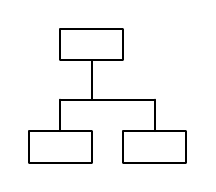
\begin{tikzpicture}[line width=1.1pt, line cap=round, line join=round, x=1mm,y=1mm]
  % Parent node.
  \draw[thick] (-7,7) rectangle (1,11);
  % Elbow connectors down to the two children.
  \draw[thick] (-3,7) -- (-3,2);
  \draw[thick] (-7,2) -- (5,2);
  \draw[thick] (-7,2) -- (-7,-2);
  \draw[thick] (5,2) -- (5,-2);
  % Children.
  \draw[thick] (-11,-6) rectangle (-3,-2);
  \draw[thick] (1,-6) rectangle (9,-2);
\end{tikzpicture}
\end{document}
